\chapter{Literature Review\label{cha:chapter2}}

This section explains the important definitions and previous research on start-ups and spin-offs to
gain better understanding of purpose of this research.

\section{Definitions of Start-Ups \label{sec:defs}}
According to \textbf{Wikipedia} \cite{6}:
``A startup company (startup or start-up) is an entrepreneurial venture which is typically a newly
emerged, fast-growing business that aims to meet a marketplace need by developing or offering an
innovative product, process or service.''
\\
\\
According to Steve Blank \cite{8}:
``A startup is a temporary organization designed to search for a repeatable and scalable business
model''.
\\
\\
``A startup is a company working to solve a problem where the solution is not obvious and success
is not guaranteed,'' says Neil Blumenthal, co-founder and co-CEO of Warby Parker \cite{9}.
\\
\\
TechCrunch writer Alex Wilhelm defines startup by ``50-100-500'' rule as follows:
``If your company has, or is any of the following, you have to hang up your Startup Uniform, and
realize that you are just another technology company either hunting for or actively avoiding an
IPO," Wilhelm writes. "\$50 million revenue run rate (forward 12 months); 100 or more
employees;Worth more than \$500 million, on paper or otherwise.'' \cite{10}
\\
\\
In a nutshell, there exists no single definition of start-up. Having read many definitions and views of
people about start-ups, I have come up with my own definition:
\\
\\
\textbf{``A start-up is an entrepreneurial venture aimed at creating value for itself and its customers by
solving a specific problem and embracing risks and failures on its way to become a stable business.
It is the outcome of efforts of individuals who work on their own resources without inheriting any
support from other organizations.''}
\\
\\

\newpage

\section{Definitions of Spin-Offs\label{sec:defs_spinoffs}}

According to \textbf{Wikipedia}\cite{7}:
\\
``Spin-offs are divisions of companies or organizations that then become independent businesses
with assets, employees, intellectual property, technology, or existing products that are taken from
the parent company.''
\\
\\
According to \textbf{Merriam Webster Dictionary} \cite{11}:
\\
``spin-off is the distribution by a business to its stockholders of particular assets and especially of
stock of another company; also: the new company created by such a distribution''
\\
\\
\textbf{The Economist Group Limited} published in blog ``\textbf{The art of the spin-off}'' \cite{12}:
\\
``In business, spin-offs are the offspring of established companies. You take a division and turn it
into a free-standing firm.''
\\
\\
A number of other studies define a spin-off as a firm whose intellectual capital originates in its
parent, for example, a university, research institute, or another companies \cite{13}.
The definition of spin-off varies depending upon the type of spin-off we are referring to. Broadly
speaking, there are two types of spin-offs i.e. Academic spin-offs and Corporate spin-offs. These
two types are further classified by researchers based on resource transfer, parental support and
reasons of their creation \cite{14}
\section{Previous Research on Start-Ups\label{sec:previous_r_startups}}
Research on Start-ups have been going on since 1980’s. The
relationship between innovativeness and success of firms has been the focus of research in literature
for many decades. Schumpeter \cite{16} described that innovativeness increased market power of a firm.
Porter \cite{17} explained that innovation improved the ability of firms to break competition. Zahra
and George \cite{18} had credited innovativeness for enhancing absorptive capacity of a company.
\\
\\
However, a lot of researchers also described negative affects of innovativeness. Samuelsson and
Davidsson \cite{19} stated that innovations could lead to introducing risks in success of start-ups.
Amason, Shrader and Tompson \cite{20} had declared innovativeness and novelty a great liability in the
path of start-ups’ success . John Freeman and Jerome S. Engel \cite{15} had compared start-ups with
corporate companies in their innovation models. According to them, big companies have
more capital, scientists and engineers, brand presence, strategic alliances, evolving organizational
structures, and well established business processes. On the other hand, young firms are a victim of
newness and are at higher risks of failure in the beginning. However, they have also mentioned that
big companies can fail in developing innovative products due to immobility in resources and
misalignment of incentives. In such scenarios, start-ups could evolve into sustainable, growing and
profitable businesses. Ari Hyytinen , Mika Pajarinen and Petri Rouvinen \cite{21} suggested that a
startup's innovativeness might in fact hurt its survival prospects. Their research has found that
survival rate for innovative startups is approximately 6–7 percentage points lower than that of non-
innovators. They also find that the interaction of innovativeness and entrepreneurs' greater appetite
for risk further reduces the prospects for survival.
\\
\\
In view of extensive research on finding affects of innovativeness on start-ups, it seems
that innovation might have either a positive or negative affect on start-ups’ success rate.
However, empirical literatures mostly states that results are positive \cite{21}.
\section{Previous Research on Spin-Offs\label{sec:previous_r_spin}}
No one can deny the importance of spin-offs in recent economic developments. Forbes calculates
that American companies completed more than 80 spin-offs worth at least \$500m each between
2002 and 2012 \cite{12}.There has been research on understanding corporate spin-offs topology \cite{23}. 
Helmut and Mike \cite{24} studied topology of spin-offs with respect to their environmental contexts as
shown in figure \ref{fig1} and defined four types of spin-offs i.e. Academic spin-off, Corporate spin-off,
Privatization buyout/buy-in of university research and Management buy-out/buy-in of division.

\begin{figure}[htb]
	\centering
	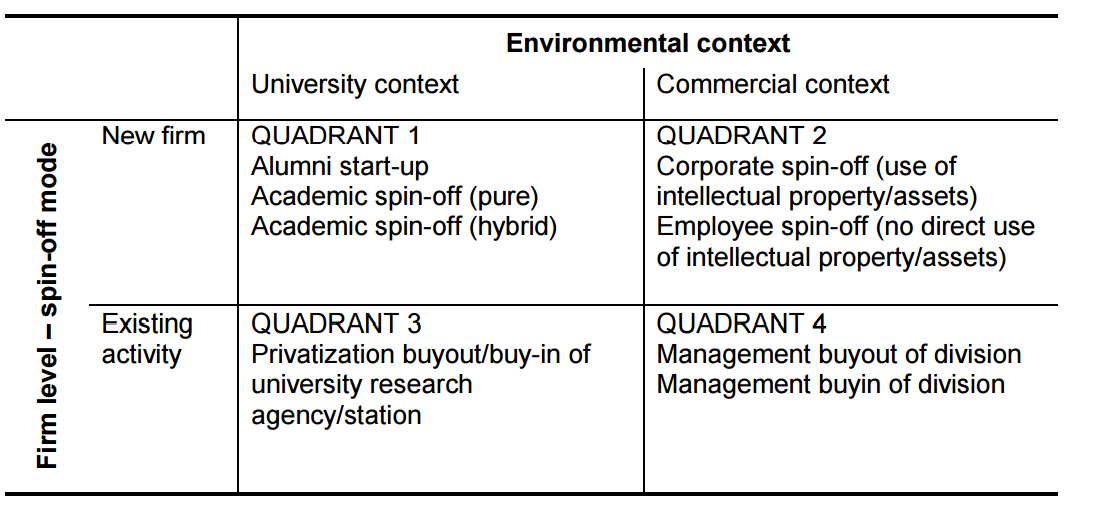
\includegraphics[width=10cm]{fig1}
	\caption{Topology of spin-offs. Adapted from ``The origin of spin-offs: a typology of corporate and academic spin-offs.'' by Fryges, Helmut, and Mike Wright. Small Business Economics 43.2 (2014)}
	\label{fig1}
\end{figure}

Sierdjan Koster did a survey of the founders of new companies and found that existing companies
had a positive impact on creation of new businesses and provides a basis for the new company to
build on. However, supported companies are less innovative \cite{50}.
\\
\\
In 1999, Institute for Prospective Technological Studies (IPTS) delivered a report ``The Impact of
Corporate Spin-Offs on Competitiveness and Employment in the European Union'' in which seven
countries were investigated ( United Kingdom, Sweden, Spain, Italy, Germany, France, and
Denmark ) based on two types of Corporate Spin-offs i.e. Restructuring-driven Spin-Off and
Entrepreneurial Spin-Offs \cite{26}. The results have shown that Corporate Spin-Off processes represent
a valuable mechanism for the transfer of technological and business knowledge and can produce
considerable impacts on competitiveness and the socio-economic environments. 
\\
\\
Andreas Stephan, in his research \cite{22}, compared research-based spin-offs with comparable knowledge-intensive firms
created in other ways. He found that out of 121 research spin-offs investigated have more patent
applications and more radical product innovations, on average, compared to similar firms.
Research has also been done in understanding the taxonomies of research-based spin-offs based on
type of resources, the business model and institutional links \cite{27}. Guido Buenstorf \cite{28} has compared
characteristics of spin-offs formed on basis of triggering events as necessity and opportunity spin-
offs. He described four types of useful knowledge which employees can learn in parent
companie i.e. knowledge about technology, markets and customer needs, organizational
processes, and personal skills.

\section{Previous Research on Comparison of Spin-Offs with Start-Ups\label{sec:previous_r_comparison}}
Peter and Viliam \cite{29} provided a theoretical framework for comparing start-ups and spin-offs in
terms of different types of support they need. James and Dennis \cite{31} had done research on different forms of incentives ,in form of property rights
and sufficient funds, faced by employees and employers which results in creation of either a start-up
or a spin-off.
Sierdjan Koster \cite{30} has compared start-ups and spin-offs based on resource theory using empirical
study of American entrepreneurs and showed that spin-offs are indeed a step ahead of firms that do
not receive support from a third party company. He identified four different types of firms based on
resource sharing and parental support as shown in figure \ref{fig2} .
\begin{figure}[htb]
	\centering
	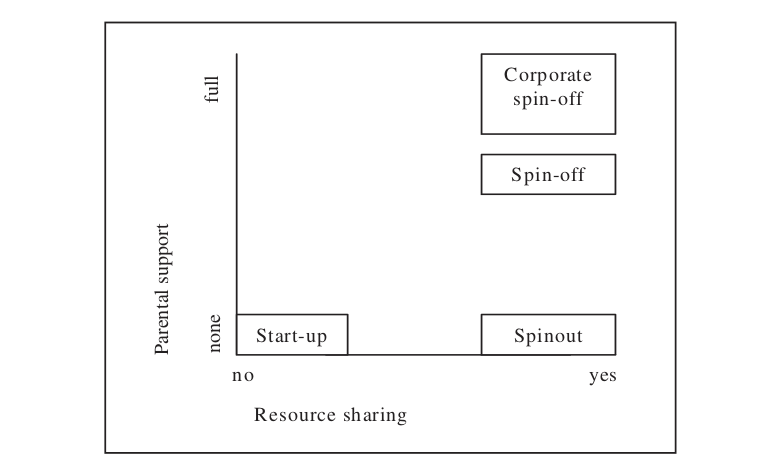
\includegraphics[width=8cm]{fig2}
	\caption{Difference between Start-up and spin-off based on resource and parental support. Adapted from ``Spin-off firms and individual start-ups. Are they really different?.'' by Sierdjan Koster. ERSA conference papers (2004)}
	\label{fig2}
\end{figure}

\begin{comment}

\begin{table}[htb]
\centering
\begin{tabular}[t]{|l|l|l|l|}
\hline
Name & Vendor & Release Year & Platform \\
\hline
\hline
A & Microsoft & 2000 & Windows \\
\hline
B & Yahoo! & 2003 & Windows, Mac OS \\
\hline
C & Apple & 2005 & Mac OS \\
\hline
D & Google & 2005 & Windows, Linux, Mac OS \\
\hline
\end{tabular}
\caption{Comparison of technologies}
\label{tab:enghistory}
\end{table}

\section{Standardization \label{sec:standard}}

This sections outlines standardization approaches regarding X.

\subsection{Internet Engineering Task Force\label{sec:itu}}

The IETF defines SIP as '...' \cite{rfcsip}

\subsection{International Telecommunication Union\label{sec:itu}}

Lorem Ipsum...

\subsection{3GPP\label{sec:3gpp}}

Lorem Ipsum...

\subsection{Open Mobile Alliance\label{sec:oma}}

Lorem Ipsum...

\section{Concurrent Approaches \label{sec:summ}}

There are lots of people who tried to implement Component X. The most relevant are ...
\end{comment}